\section{Beschreibung der Hardware}
\label{beschreibung_hardware}
\subsection{Intel Galileo Gen2}

\begin{wrapfigure}{r}{0.6\textwidth}
\centering
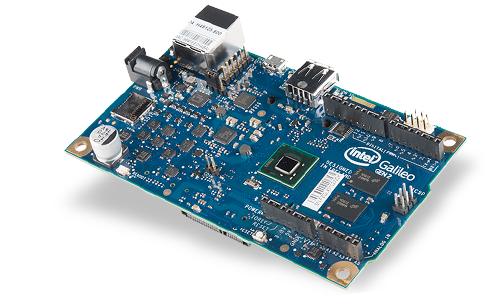
\includegraphics[scale=0.5]{images/iot_galileo.png}
\caption{Intel Galileo Gen2\cite{intel_galileo_image}}
\label{fig:Intel Galileo Gen2}
\end{wrapfigure}

Das Galileo Developer Board\cite{intel_datasheet_galileo} der zweiten Generation von
Intel ist ein SoC und besitzt einen Intel® Quark™ SoC X1000 Prozessor. Die Architektur des 32bit Prozessor basiert auf x86\cite{intel_datasheet} und somit ist das Galileo
Board eines der wenigen, auf denen ein CISC-Prozessor verbaut wurde. Die Hardware
besitzt keinen Videoausgang. Es ist also nur möglich, über eine RS232 Schnittstelle oder über Ethernet,
eine Verbindung zum System zu erstellen. Die GPIO Ein- und Ausgänge sind über den
PCI-Bus verbunden. Somit ist es sehr schwer, den GPIO ohne passenden Treiber oder
Softwareschicht anzusprechen. Im Vergleich sind die GPIO des RaspberryPI, das als zweites Board gewählt wurde,
direkt über eine Speicheradresse ansprechbar.
\par
Von Intel wird ein angepasstes Betriebssystem als fixfertiges Image angeboten. Dieses System basiert auf
der Linux Distribution Yocto. Es sind aber auch inoffizielle Debian Distributionen im
Internet erhältlich. Der Vorteil von Debian gegenüber der offiziellen Version, ist die
grössere Verbreitung und die damit verbundenen Hilfestellungen im Internet. Das Cross-Compiling eines Kernelmoduls scheint so einfacher als auf der Yocto-Distribution.


\subsection{RaspberryPi}


\begin{wrapfigure}{r}{0.6\textwidth}
\centering
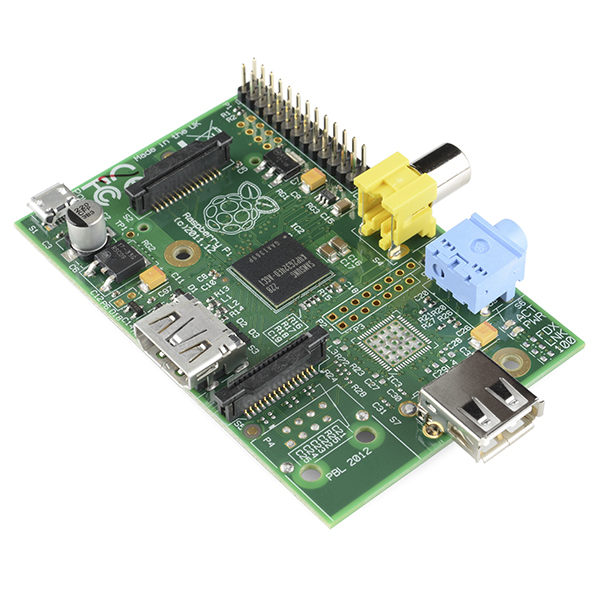
\includegraphics[scale=0.4]{images/raspberry-pi-2.png}
\caption{Raspberry Pi 1 A\cite{raspberry_image}}
\label{fig:Raspberry Pi 1 A}
\end{wrapfigure}


Als zweites Experimentier-Board wird das Raspberry Pi Model B\cite{raspberry_foundation} verwendet. Das Board wird von der Raspberry Pi Foundation betrieben. Das Modell besitzt einen Broadcom BCM2835\cite{broadcom_datasheet} Chip. Der darin verbaute Prozessor wurde von der Firma ARM unter dem Namen ARM1176JZFS\cite{arm_datasheet} (ARM11) spezifiziert. Die Software muss für die Architektur ARMv6 kompiliert werden. Im Gegensatz zum Galileo Board von Intel ist der Prozessor ein RISC-CPU. Beide Boards haben eine 32bit Adressierung.
\par
Eine Remote-Verbindung lässt sich über eine serielle Schnittstelle oder über Ethernet realisieren. Durch das Vorhandensein eines Videoausgangs und eines USB-Anschlusses würde sich das Raspberry Pi auch direkt über Monitor und Tastatur bedienen lassen. Die GPIOs sind direkt über die Speicheradressierung ansprechbar. Somit wäre eine Erweiterung des Benchmarks, der in Assembler geschrieben ist, durchaus denkbar. So könnten auf einfache Weise weitere Messungen über die GPIO erfolgen. Das offizielle Betriebssystem der Foundation ist ein Debian basiertes OS mit dem Name Raspbian. Zusätzlich werden als Third-Party Produkte weitere unterschiedliche Betriebssysteme zur Verfügung gestellt. 











